% 导言区

\documentclass{ctexart} %ctexbook,ctexrep
\usepackage{graphicx}
\graphicspath{{figures/}} % 指定图片的目录。目录用大括号括开。

%\usepackage{ctex}

% 正文区(文稿区)
%\tabular 关键字。 l,c.r,p.来进行设置表格形式。



\begin{document}
	\LaTeX{}中的插图:小姑娘,见图
	\ref{fig-girls} %交叉引用设置好的标签。
	% figure 浮动体环境。
	\begin{figure}[htbp]%参数设置浮动体排版的位置。
		% 采用centering命令行让环境的内容居中排版。
		\centering
		
\includegraphics[scale=0.3]{girls} 
		
		\caption{\TeX 美女小姑娘}
		\label{fig-girls} %设定一个标签,方便之后的交叉引用。
		%将图片放在figure环境中。
	\end{figure}
	
	
	我们看到,图\ref{fig-girls2} 中的美女要比图\ref{fig-girls} 中的美女漂亮的多。
	\begin{figure}[htbp]%参数设置浮动体排版的位置。
		% 采用centering命令行让环境的内容居中排版。
		\centering
		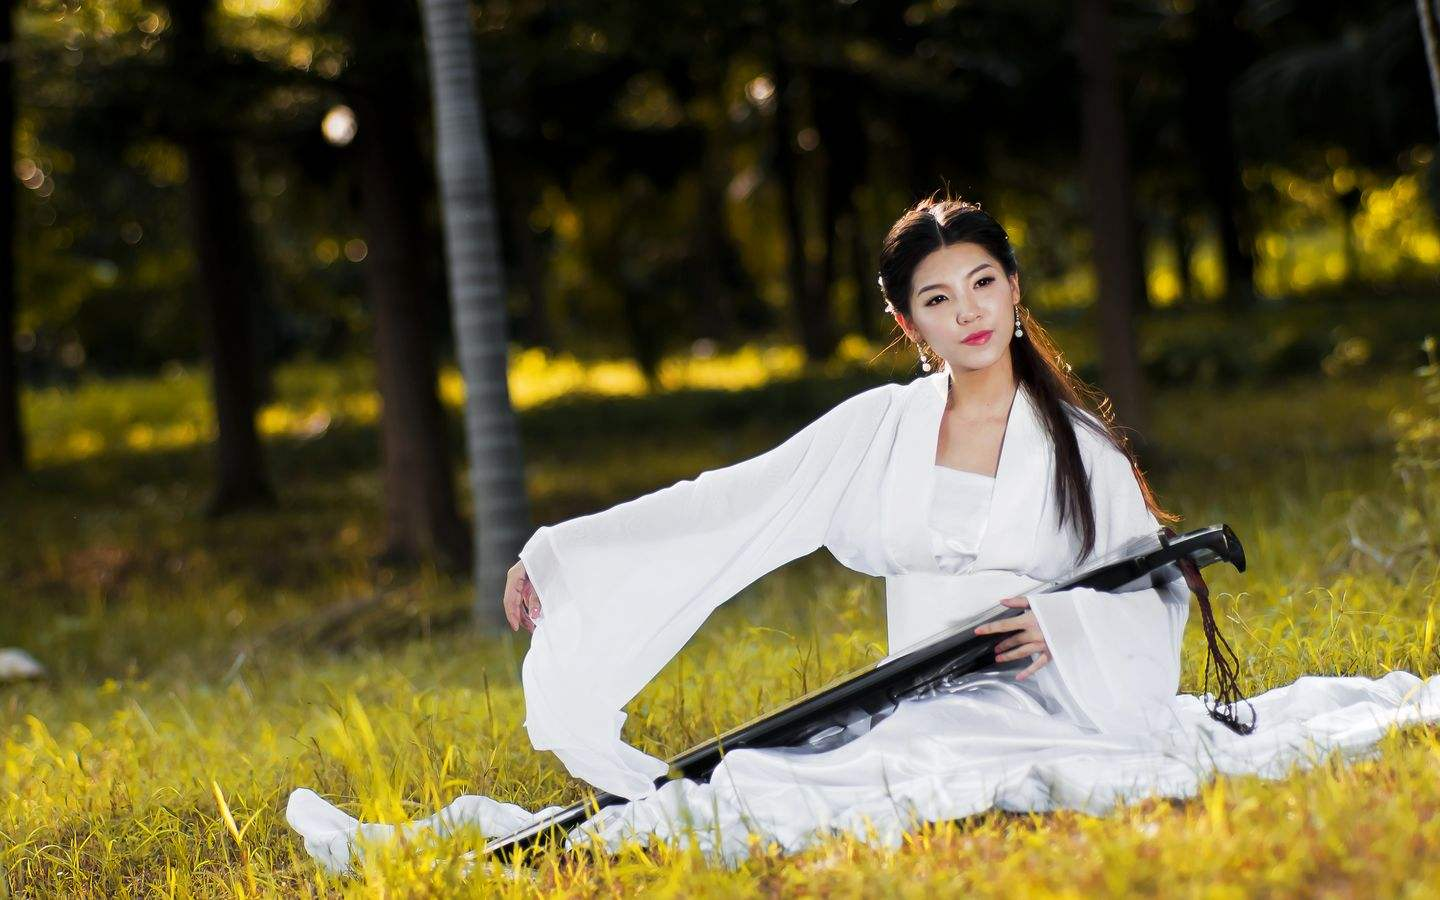
\includegraphics[scale=0.2]{girls2} 
		
		\caption{\TeX 美女小姑娘2}
		\label{fig-girls2} %设定一个标签,方便之后的交叉引用。
		%将图片放在figure环境中。
	\end{figure}
	
	在\LaTeX{} 中的表格:如表 \ref{tab-chengjidan}
	%table 浮动提环境。将表格放到环境中。
	\begin{table}[h]
		\centering
		\caption{成绩单}
		\label{tab-chengjidan}
		\begin{tabular}{l ||c |c |c |p{1.5cm}}
			\hline \hline
			姓名 & 语文 & 数学 & 外语 & 备注\\
			\hline
			张三 & 89 & 100 & 70 & 优秀\\
			张三 & 89 & 100 & 70 & 优秀\\
			张三 & 89 & 100 & 70 & 优秀\\
			张三 & 89 & 100 & 70 & 优秀\\
			
			\hline
			\hline
		\end{tabular}
	\end{table}
	
\end{document}

% 由p产生的内容,当内容超过时,自动换行。
% texdoc booktab 查看相应文档设置。
% texdoc longtab 跨页长表格。
% texdoc tabu 综合表格宏包